\documentclass[preprint,12pt,aps,pra,showkeys,amsmath,amssymb,superscriptaddress,floatfix]{revtex4-2}
\usepackage[T1]{fontenc}
\usepackage[utf8]{inputenc}
\usepackage{amsmath,amssymb,amsthm,mathtools,mathrsfs}
\usepackage{microtype,booktabs,enumitem}
\usepackage{xcolor,tikz,etoolbox}
\usepackage[skins,breakable]{tcolorbox}
\usepackage{needspace}
% Keep diagram geometry independent of REVTeX preprint body spacing.
\AtBeginEnvironment{tikzpicture}{\linespread{1}\selectfont}
\usetikzlibrary{arrows.meta,positioning,calc,fit,decorations.pathreplacing}
\usepackage{graphicx}
\usepackage{hyperref}

\definecolor{MMBlue}{RGB}{0,82,155}
\definecolor{MMOrange}{RGB}{200,80,0}
\tikzset{
 mmnode/.style={draw=MMBlue,rounded corners=2pt,fill=MMBlue!4,align=left,execute at begin node={\raggedright},text width=5cm,font=\fontsize{10}{12}\selectfont,inner sep=6pt},
 mmimport/.style={mmnode,draw=black!65,fill=black!4},
 mmcandidate/.style={mmnode,draw=MMOrange,dashed,fill=MMOrange!5},
 mmrejected/.style={mmnode,draw=black,densely dotted,fill=black!8},
 mmproof/.style={->,thick,MMBlue},
 mmflow/.style={->,semithick,black!70},
 mmrepair/.style={->,dashed,thick,MMOrange},
 mmcandidatearrow/.style={->,dashed,semithick,MMOrange},
 mmnote/.style={font=\scriptsize,fill=white,inner sep=2pt,align=center}}

\usepackage[section]{placeins}
\setlength{\emergencystretch}{3em}
\setlist{itemsep=3pt,topsep=4pt}
\newtheorem{theorem}{Theorem}[section]
\newtheorem{proposition}[theorem]{Proposition}
\newtheorem{lemma}[theorem]{Lemma}
\newtheorem{corollary}[theorem]{Corollary}
\theoremstyle{definition}
\newtheorem{definition}[theorem]{Definition}
\newtheorem{example}[theorem]{Example}
\theoremstyle{remark}
\newtheorem{remark}[theorem]{Remark}
% Avoid isolated statement headings and single-line paragraph fragments.
\BeforeBeginEnvironment{theorem}{\Needspace{6\baselineskip}}
\BeforeBeginEnvironment{definition}{\Needspace{5\baselineskip}}
\BeforeBeginEnvironment{proposition}{\Needspace{5\baselineskip}}
\BeforeBeginEnvironment{lemma}{\Needspace{5\baselineskip}}
\BeforeBeginEnvironment{corollary}{\Needspace{5\baselineskip}}
\clubpenalty=5000
\widowpenalty=5000
\newcommand{\R}{\mathbb R}\newcommand{\Z}{\mathbb Z}\newcommand{\N}{\mathbb N}
\newcommand{\Pa}{\operatorname{Pa}}\newcommand{\Desc}{\operatorname{Desc}}
\newcommand{\cl}{\operatorname{cl}}\newcommand{\cost}{\operatorname{cost}}
\newcommand{\status}{\operatorname{status}}
% Faculty cards: a visual rail groups the five faculties within one agent.
% The rail has no arrowhead and does not represent a proof dependency.
\newcommand{\mmfacultybadge}[1]{%
 \node[circle,draw=MMBlue,line width=1pt,fill=white,
 minimum size=7mm,inner sep=0pt,font=\sffamily\small\bfseries,text=MMBlue]
 at ([xshift=15pt,yshift=-15pt]frame.north west) {#1};}
\newcommand{\mmfacultyrail}{%
 \draw[MMBlue!80,line width=1pt]
 ([xshift=15pt,yshift=2pt]frame.north west)--
 ([xshift=15pt,yshift=-2pt]frame.south west);}
\newtcolorbox{mmfacultybox}[2]{enhanced,breakable,
 colback=MMBlue!4,colframe=MMBlue!4,boxrule=0pt,arc=3pt,
 left=39pt,right=9pt,top=4pt,bottom=4pt,
 before skip=2pt,after skip=2pt,
 fontupper=\small\linespread{1.1}\selectfont,
 overlay unbroken={\mmfacultyrail\mmfacultybadge{#1}},
 overlay first={\mmfacultyrail\mmfacultybadge{#1}},
 overlay middle={\mmfacultyrail},overlay last={\mmfacultyrail}}
\newcommand{\mmfaculty}[3]{%
 \begin{mmfacultybox}{#1}{#2}
 {\sffamily\bfseries\color{MMBlue}#2}\par\smallskip #3
 \end{mmfacultybox}}
\newcommand{\agent}[9]{%
 \Needspace{8\baselineskip}
 \subsubsection{#1}
 \noindent\textbf{Object.} #2\par
 \noindent\textbf{Role.} #3\par\smallskip
 \mmfaculty{E}{Ego}{#4}
 \mmfaculty{M}{Memory}{#5}
 \mmfaculty{I}{Intellect}{#6}
 \mmfaculty{S}{Sense}{#7}
 \mmfaculty{A}{Action}{#8}
 \smallskip\noindent #9\par}

\usepackage{longtable,array,calc}
\providecommand{\tightlist}{\setlength{\itemsep}{2pt}\setlength{\parskip}{0pt}}
\makeatletter
\def\frontmatter@abstract@produce{\par\addvspace{\frontmatter@preabstractspace}%
\begingroup\prep@absbox\unvbox\absbox\post@absbox\endgroup
\addvspace{\frontmatter@postabstractspace}}
\makeatother
\newcommand{\field}[2]{\par\smallskip\noindent\textbf{#1.} #2\par}
\setlength{\emergencystretch}{5em}
\AtBeginEnvironment{verbatim}{\small\linespread{1.0}\selectfont}


\hypersetup{colorlinks=true,linkcolor=MMBlue,urlcolor=MMBlue,pdfauthor={Dibakar Sigdel}}

\begin{document}

\title{The Two Borel--Cantelli Lemmas\\[4pt]\large An End-to-End Meta-Math Walkthrough}

\author{Dibakar Sigdel}

\affiliation{Mindverse Computing LLC, Lynnwood, WA 98087, USA}

\date{October 2026}

\begin{abstract}

The summable case bounds the entire tail union. The independent
divergent case instead bounds the probability that an entire long tail
block contains no occurrence. The report presents the target theorem,
declared imports, a dependency graph, five-faculty node contracts, a
continuous proof, a worked example, and a hypothesis-repair audit. It is
an authored mathematical exposition, not a deployed-agent transcript or
a formal proof-assistant certificate.

\end{abstract}\maketitle\linespread{1.12}\selectfont

\noindent\textbf{PS-01 / Probability and Stochastic Processes / Report v1}

\section{Target and import contract}

\begin{theorem}

For events \(A_n\) on a probability space, write
\(\{A_n\text{ i.o.}\}=\bigcap_{N\ge1}\bigcup_{n\ge N}A_n\). Prove: (i)
if \(\sum_n\mathbb P(A_n)<\infty\), then
\(\mathbb P(A_n\text{ i.o.})=0\); (ii) if the events are mutually
independent and \(\sum_n\mathbb P(A_n)=\infty\), then
\(\mathbb P(A_n\text{ i.o.})=1\). Mutual independence means every finite
subcollection has product probability, including the corresponding
complements.

\end{theorem}

\subsection{Foundations and permitted imports}

Use countable subadditivity, continuity of probability along monotone
event sequences, finite-product independence, and \(1-p\le e^{-p}\) for
\(0\le p\le1\). These follow respectively from countable additivity and
elementary real analysis. The first direction has no independence
assumption.

\clearpage\section{Node interaction workflow}

\begin{center}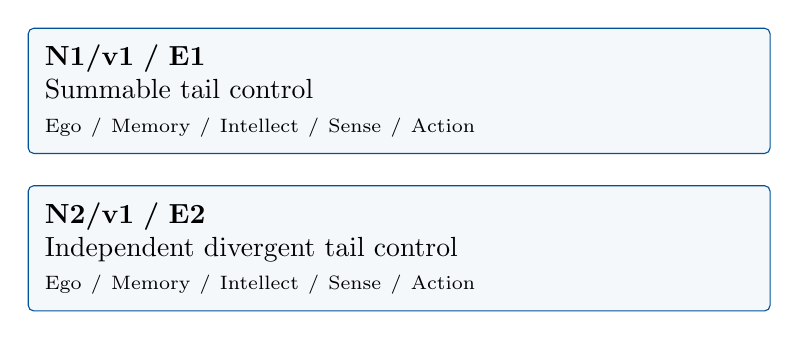
\begin{tikzpicture}[>=Stealth,x=1cm,y=1cm]

\node[mmnode,text width=9cm,minimum height=1.25cm] (N1) at (0,0.0) {\textbf{N1/v1 / E1}\\Summable tail control\\{\scriptsize Ego / Memory / Intellect / Sense / Action}};

\node[mmnode,text width=9cm,minimum height=1.25cm] (N2) at (0,-2.0) {\textbf{N2/v1 / E2}\\Independent divergent tail control\\{\scriptsize Ego / Memory / Intellect / Sense / Action}};

\end{tikzpicture}\end{center}

Each box is one mathematical agent containing all five faculties. Blue
arrows carry the versioned exports listed below. The layout gives a
reading order; only drawn arrows assert dependencies. Diagnostic repair
is separate from the proof DAG.

\subsection{Versioned evidence-transfer ledger}
No inter-node proof imports are needed: the nodes establish separate directions under the common theorem contract.


\begingroup\small\linespread{1.05}\selectfont

\endgroup

\clearpage\section{Agent roles and five-faculty activities}\begingroup\small\linespread{1.05}\selectfont\setlist{itemsep=1pt,topsep=2pt}

\subsection{N1/v1: Summable tail control}

\field{Object and role}{Bound a tail union and let the summable tail vanish. \textbf{Local
obligation:} Under summability, \(\mathbb P(A_n\text{ i.o.})=0\).}

\field{Inputs}{\(\sum_n\mathbb P(A_n)<\infty\) and \(B_N=\bigcup_{n\ge N}A_n\).}

\mmfaculty{E}{Ego}{Publish E1/v1 only after establishing this obligation: Under
summability, \(\mathbb P(A_n\text{ i.o.})=0\).}

\mmfaculty{M}{Memory}{\(\sum_n\mathbb P(A_n)<\infty\) and \(B_N=\bigcup_{n\ge N}A_n\). Retain
the stated assumptions and import versions.}

\mmfaculty{I}{Intellect}{Bound a tail union and let the summable tail vanish.}

\mmfaculty{S}{Sense}{No products or independence are used in this direction.}

\mmfaculty{A}{Action}{Carry out activities N1.1--N1.2 below, retaining each calculation and
construction as evidence.}

\smallskip\noindent\textbf{Numbered mathematical activities}

\begin{enumerate}[label=N1.\arabic*,leftmargin=3.4em]

\item Countable subadditivity gives
\(\mathbb P(B_N)\le\sum_{n\ge N}\mathbb P(A_n)\). The right side tends
to zero because the series converges.

\item The events \(B_N\) decrease and their intersection is the
infinitely-often event. Continuity from above yields its probability as
\(\lim_N\mathbb P(B_N)=0\).

\end{enumerate}

\field{Export E1/v1}{Under summability, \(\mathbb P(A_n\text{ i.o.})=0\).}

\field{Acceptance gate}{No products or independence are used in this direction.}

\field{Targeted repair}{If independence is imposed in this branch, remove it from the local
inputs: the union bound already supplies the full conclusion. Withhold
this export and recheck its descendants after a versioned correction.}

\clearpage

\subsection{N2/v1: Independent divergent tail control}

\field{Object and role}{Estimate the complementary event of no occurrence in a finite tail block
and then exhaust the tail. \textbf{Local obligation:} Under independence
and divergence, \(\mathbb P(A_n\text{ i.o.})=1\).}

\field{Inputs}{Mutual independence and \(\sum_n\mathbb P(A_n)=\infty\).}

\mmfaculty{E}{Ego}{Publish E2/v1 only after establishing this obligation: Under
independence and divergence, \(\mathbb P(A_n\text{ i.o.})=1\).}

\mmfaculty{M}{Memory}{Mutual independence and \(\sum_n\mathbb P(A_n)=\infty\). Retain the
stated assumptions and import versions.}

\mmfaculty{I}{Intellect}{Estimate the complementary event of no occurrence in a finite tail block
and then exhaust the tail.}

\mmfaculty{S}{Sense}{Divergence of the series alone does not give the finite product
identity; mutual independence is used there.}

\mmfaculty{A}{Action}{Carry out activities N2.1--N2.2 below, retaining each calculation and
construction as evidence.}

\smallskip\noindent\textbf{Numbered mathematical activities}

\begin{enumerate}[label=N2.\arabic*,leftmargin=3.4em]

\item Fix \(N\). For \(m\ge N\), independence gives
\(\mathbb P(\bigcap_{n=N}^m A_n^c)=\prod_{n=N}^m(1-\mathbb P(A_n))\le\exp(-\sum_{n=N}^m\mathbb P(A_n))\).
Divergence makes this tend to zero as \(m\to\infty\).

\item By continuity from above, \(\mathbb P(\bigcap_{n\ge N}A_n^c)=0\), so
\(\mathbb P(B_N)=1\). The intersection of the countably many
probability-one events \(B_N\) still has probability one, proving the
second assertion.

\end{enumerate}

\field{Export E2/v1}{Under independence and divergence, \(\mathbb P(A_n\text{ i.o.})=1\).}

\field{Acceptance gate}{Divergence of the series alone does not give the finite product
identity; mutual independence is used there.}

\field{Targeted repair}{If the product step is used for dependent events, withhold this export
and either verify independence or use a separately justified dependence
condition. Withhold this export and recheck its descendants after a
versioned correction.}

\endgroup\clearpage\section{Continuous mathematical proof}\label{sec:proof}

\subsection{N1 --- Summable tail
control}\label{n1-summable-tail-control}

\begin{enumerate}
\def\labelenumi{\arabic{enumi}.}
\item
  \textbf{N1.1.} Countable subadditivity gives
  \(\mathbb P(B_N)\le\sum_{n\ge N}\mathbb P(A_n)\). The right side tends
  to zero because the series converges.
\item
  \textbf{N1.2.} The events \(B_N\) decrease and their intersection is
  the infinitely-often event. Continuity from above yields its
  probability as \(\lim_N\mathbb P(B_N)=0\).
\end{enumerate}

\subsection{N2 --- Independent divergent tail
control}\label{n2-independent-divergent-tail-control}

\begin{enumerate}
\def\labelenumi{\arabic{enumi}.}
\item
  \textbf{N2.1.} Fix \(N\). For \(m\ge N\), independence gives
  \(\mathbb P(\bigcap_{n=N}^m A_n^c)=\prod_{n=N}^m(1-\mathbb P(A_n))\le\exp(-\sum_{n=N}^m\mathbb P(A_n))\).
  Divergence makes this tend to zero as \(m\to\infty\).
\item
  \textbf{N2.2.} By continuity from above,
  \(\mathbb P(\bigcap_{n\ge N}A_n^c)=0\), so \(\mathbb P(B_N)=1\). The
  intersection of the countably many probability-one events \(B_N\)
  still has probability one, proving the second assertion.
\end{enumerate}

\hfill$\square$

\section{Worked orchestration}

For independent fair coin tosses, let \(A_n\) be the event that toss
\(n\) is heads. The sum of probabilities diverges, so heads occur
infinitely often almost surely. For a separate sequence of events
\(B_n\) with \(\mathbb P(B_n)=2^{-n}\), the sum is finite, so only
finitely many \(B_n\) occur almost surely regardless of their
dependence.

\subsection{Boundary and hypothesis audit}

Let \(A_n=A\) for every \(n\), where \(\mathbb P(A)=1/2\). Then
\(\sum_n\mathbb P(A_n)=\infty\), but the infinitely-often event is just
\(A\), of probability \(1/2\). This disproves the divergent implication
without a dependence hypothesis.

\section{Illustrative failure and repair}

The following is an authored diagnostic scenario. Changed assumptions
define a new contract; they do not retroactively prove the original
statement.

\subsection{Rejected argument, diagnosis, and correction}
\textbf{Rejected N2 inference:} a divergent sum of probabilities implies
probability one of infinitely many occurrences without independence.
\textbf{Sense witness:} identical events \(A_n=A\). \textbf{Diagnosis:}
Intellect replaced the probability of an intersection by a product
without authorization. \textbf{Repair:} use mutual independence only in
the second branch, as in §1. The first branch remains valid for
arbitrary dependence; its export need not be revised.

\subsection{Publication and reuse}
The corrected export retains its explicit assumptions. A hypothetical
revision receives a new version, and each consuming activity is
rechecked; this scenario is not a recorded runtime event. \textbf{Next
direction:} Apply the summable half to error events in PS-02; the
probability bound must be summable over all sample sizes.

\par\medskip\begingroup\small\linespread{1.0}\selectfont\noindent\textbf{Provenance.} This authored proof is complete relative to its declared imports. Reuse
each export with its assumptions, proof, and version. The original
Markdown remains available for comparison.
\par\endgroup

\par\smallskip\begingroup\small\linespread{1.0}\selectfont\noindent\textbf{Further reading.} \href{https://stanford.edu/~montanar/TEACHING/Stat310A/lnotes.pdf}{Amir
Dembo, Probability Theory: STAT310/MATH230 notes} for measure-theoretic
probability and limit arguments;
\href{https://web.stanford.edu/class/stats310c/syllabus.html}{Stanford
STAT310C syllabus and lecture materials} for martingale inequalities and
stopping theorems. The versions and proofs used in this collection are
stated explicitly.\par\endgroup

\end{document}
